% !TeX program = xelatex
% 2026 年全国大学生电子设计竞赛 H 题设计报告。
% 使用 XeLaTeX 编译：latexmk -xelatex -interaction=nonstopmode main.tex
\documentclass[UTF8,a4paper,12pt]{ctexart}

\usepackage[left=2.6cm,right=2.6cm,top=3.1cm,bottom=2.5cm]{geometry}
\usepackage{amsmath}
\usepackage{array}
\usepackage{booktabs}
\usepackage{caption}
\usepackage{enumitem}
\usepackage{etoolbox}
\usepackage{fancyhdr}
\usepackage{float}
\usepackage{graphicx}
\usepackage{longtable}
\usepackage{setspace}
\usepackage{tabularx}
\usepackage{titlesec}
\usepackage[hypertexnames=false]{hyperref}

\hypersetup{hidelinks,pdftitle={车载平衡滚球运动控制系统设计报告}}
\graphicspath{{images/}}
\setlength{\parindent}{2em}
\setlength{\parskip}{0pt}
\renewcommand{\arraystretch}{1.0}
% 表格采用更紧凑字号，正文使用小四宋体并采用较紧凑的固定 18 磅行距。
\AtBeginEnvironment{tabularx}{\fontsize{10pt}{14pt}\selectfont\sloppy}
\pagestyle{fancy}
\fancyhf{}
\fancyfoot[R]{\zihao{5}\thepage}
\renewcommand{\headrulewidth}{0pt}
\renewcommand{\footrulewidth}{0pt}
\setlist[itemize]{itemsep=0.2em,topsep=0.2em}
\captionsetup{font=small,labelsep=quad}
\titleformat{\section}{\heiti\zihao{4}}{\thesection}{0.8em}{}
\titleformat{\subsection}{\heiti\zihao{-4}}{\thesubsection}{0.6em}{}
\titleformat{\subsubsection}{\heiti\normalsize}{\thesubsubsection}{0.5em}{}
\renewcommand{\contentsname}{目\quad 录}
\renewcommand{\figurename}{图}
\renewcommand{\tablename}{表}

% 若 images/system-photo.jpg 已放入目录，则在硬件设计中插入实物照片；否则保留醒目占位框。
\newcommand{\SystemPhoto}{%
  \begin{figure}[H]
    \centering
    \IfFileExists{images/system-photo.jpg}{%
      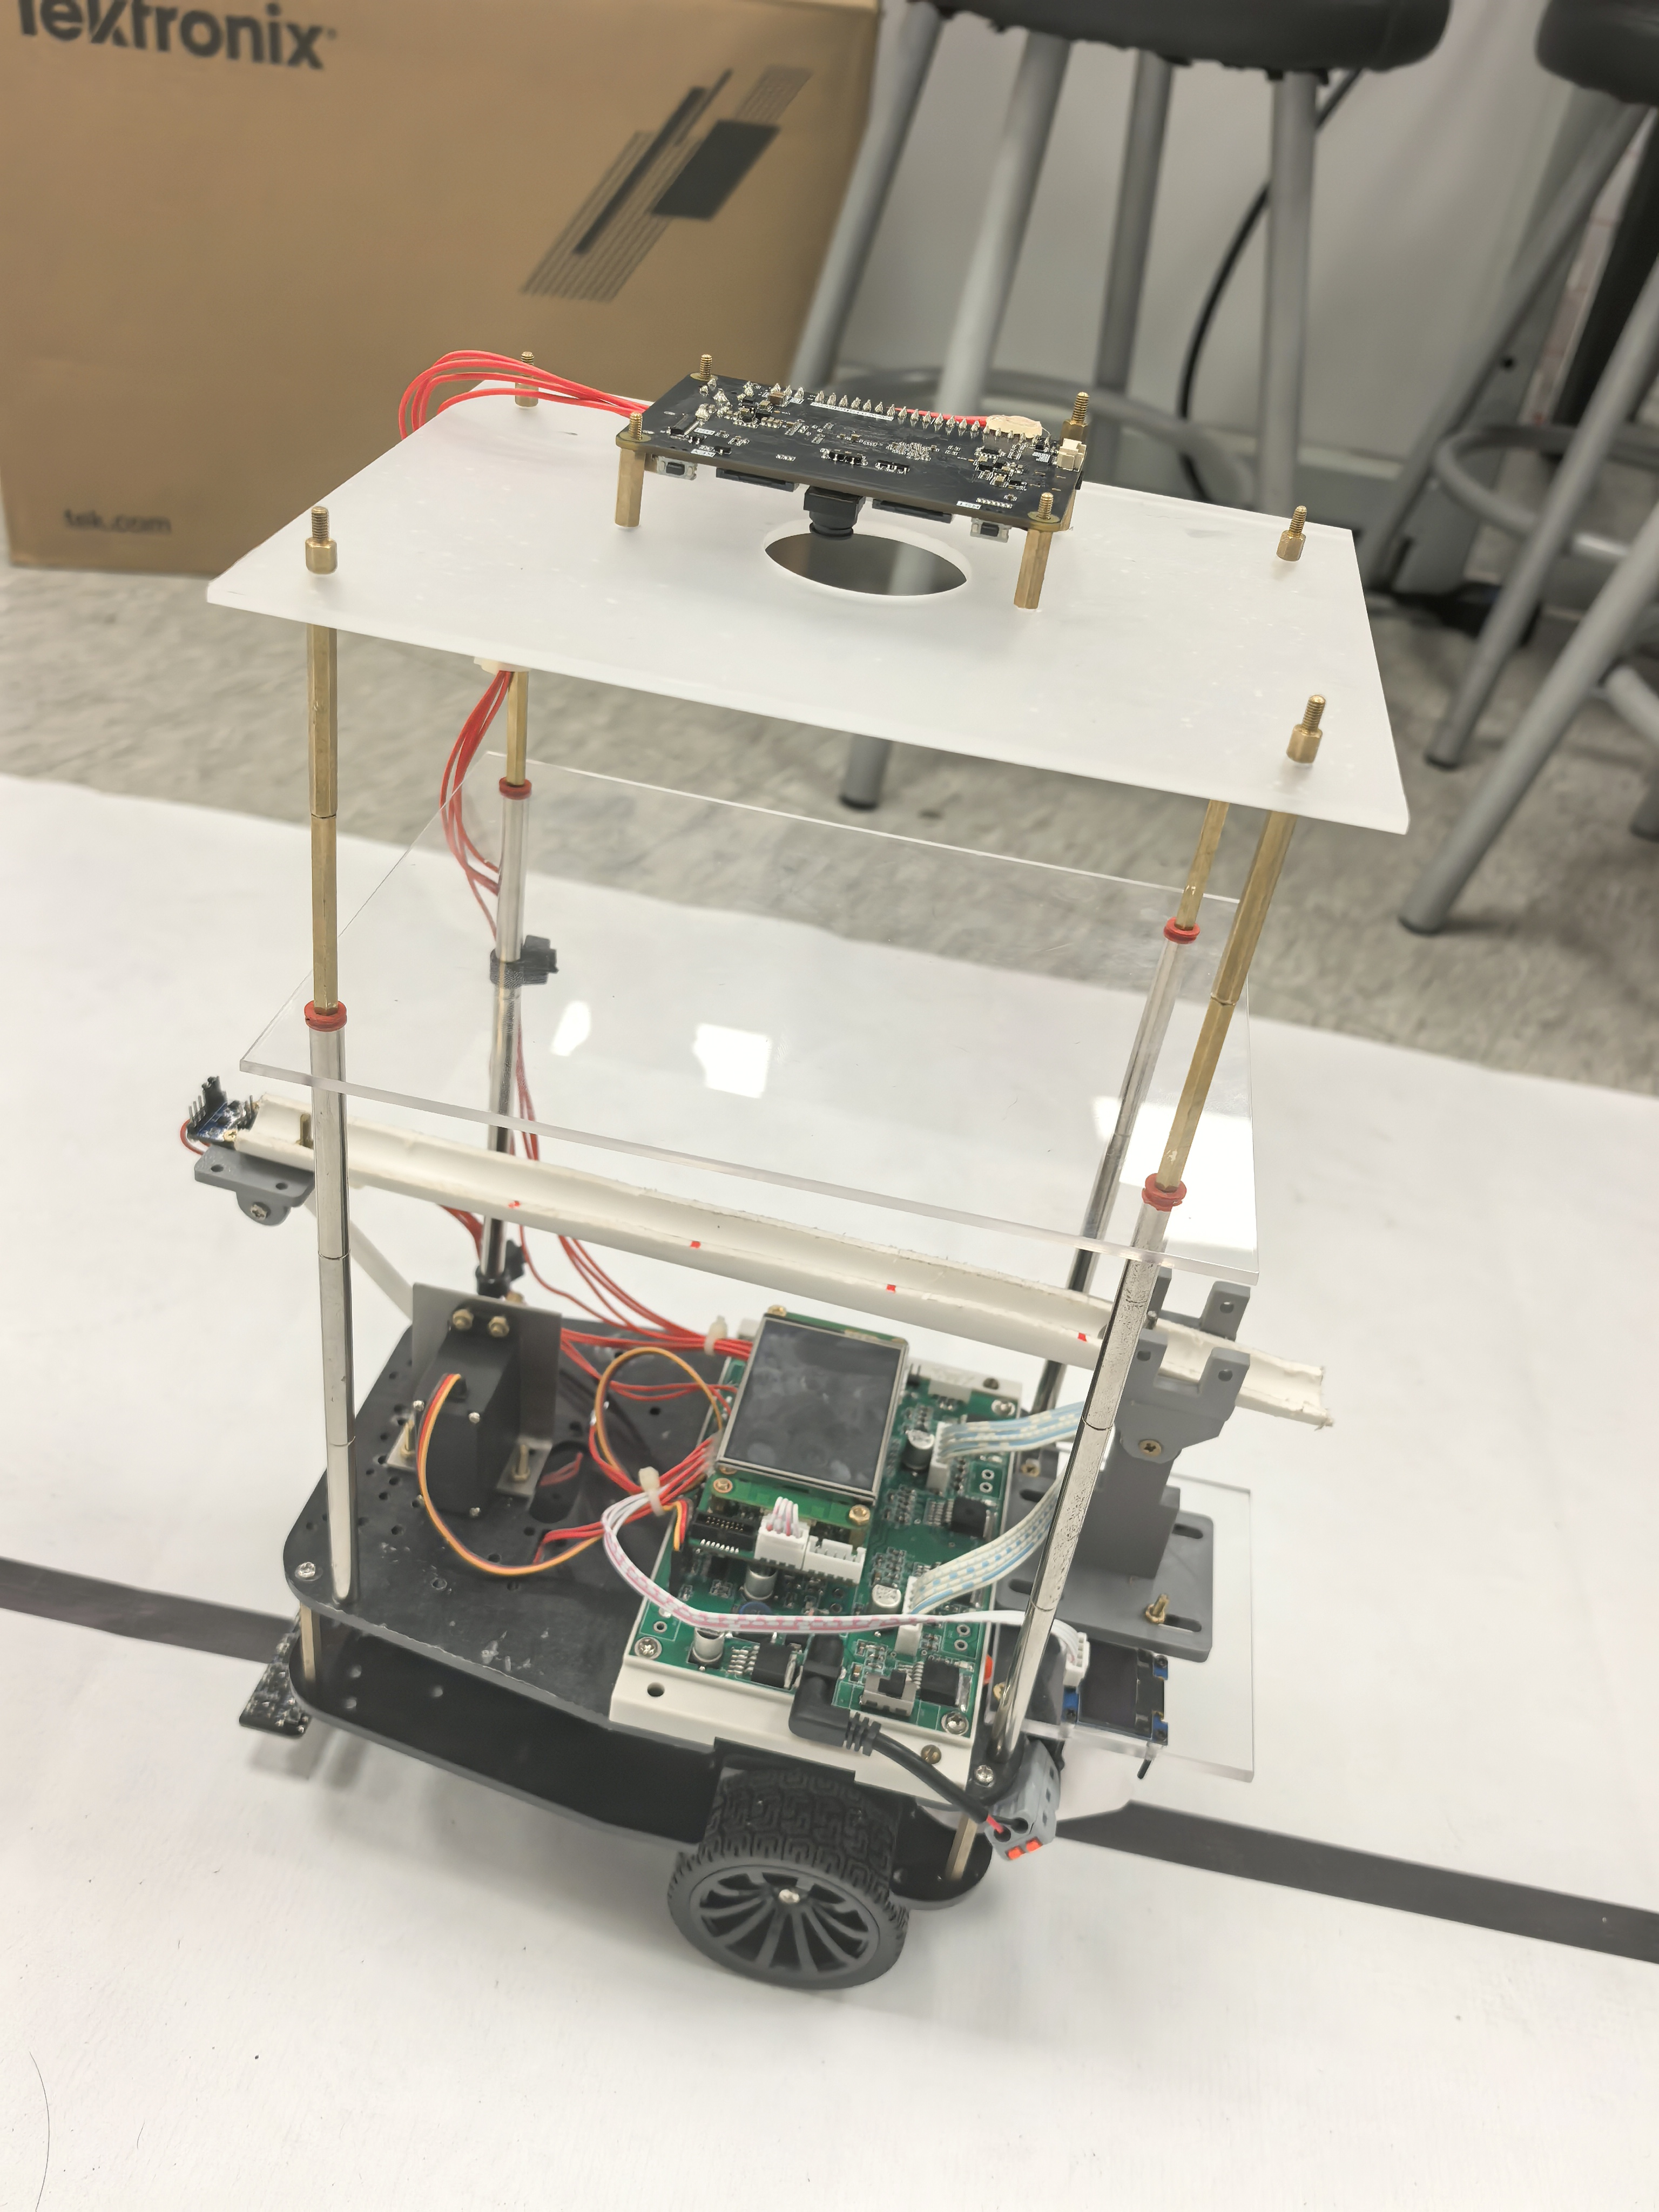
\includegraphics[height=7cm,width=0.72\textwidth,keepaspectratio]{system-photo.jpg}%
    }{%
      \fbox{\parbox[c][5.5cm][c]{0.72\textwidth}{\centering\heiti
      实物照片待放置\\[0.6em]
      请将用户提供的照片保存为\\
      \texttt{docs/images/system-photo.jpg}}}%
    }
    \caption{车载平衡滚球运动控制系统实物图}
    \label{fig:system-photo}
  \end{figure}
}

\begin{document}
\fontsize{12pt}{18pt}\selectfont
\pagenumbering{arabic}
\begin{center}
  {\zihao{3}\heiti 2026 年全国大学生电子设计竞赛\par}
  \vspace{0.35em}
  {\zihao{2}\heiti 车载平衡滚球运动控制系统\par}
  \vspace{0.15em}
  {\zihao{4}\heiti （H 题）\par}
  \vspace{0.8em}
  {\Large\heiti 摘\quad 要\par}
\end{center}

本系统以 STM32H745ZI6 为车载主控，以 CanMV K230 完成钢球识别和无线图传，采用八路红外阵列循迹，并由 LSM6DSV16X 测量管道姿态。底盘采用循迹偏差 PD 与双轮速度 PID，滚球机构采用钢球位置外环和管道姿态内环的串级控制。单连杆模型给出 70.72\,mm 连杆设计值；仿真中钢球 $0\rightarrow+5\,\mathrm{cm}\rightarrow-5\,\mathrm{cm}$ 的末端到达时间为 2.38\,s，5\,s 误差约 1.44\,mm。当前系统已完成主机侧单元测试、图传软件和部分实物验证，动态行驶平衡仍需统一机械基准、执行器映射并完成整车联调。

\noindent\textbf{关键词：}智能小车；滚球平衡；机器视觉；红外循迹；串级控制；姿态融合

\clearpage
\begingroup
  \fontsize{10pt}{14pt}\selectfont
  \tableofcontents
\endgroup
\clearpage

\section{方案设计与论证}

\subsection{任务要求与设计指标}

赛题要求小车在规定跑道上循迹行驶，同时控制直径约 10\,mm 的钢球在长 25\,cm、外径 20\,mm 的 PPR 管内稳定运动；车载摄像头同时承担钢球检测、无线实时图传、录像和回放。PPR 管铰链中心距车体安装面高度不小于 5\,cm，车体外形不大于 $35\,\mathrm{cm}\times25\,\mathrm{cm}$，循迹方式限定为红外光电模块。

据此，20\,s 和 30\,s 完成一圈所需平均速度约为 0.307\,m/s、0.205\,m/s。现有基础速度设为 0.40\,m/s，通过弯道降速、终点宽线确认和滚球稳定裕量满足时间要求。

\begin{table}[H]
  \centering
  \caption{主要设计目标与当前状态}
  \label{tab:targets}
  \begin{tabularx}{\textwidth}{>{\raggedright\arraybackslash}p{0.18\textwidth}X>{\raggedright\arraybackslash}p{0.32\textwidth}}
    \toprule
    项目 & 设计目标 & 当前状态 \\
    \midrule
    无线视频 & K230 建立热点并输出 MJPEG，可录像回放 & 软件框架已实现，待整车验证时延 \\
    单圈循迹 & 平均车速不低于 0.31\,m/s，终点误差不大于 2\,cm & 循迹与终点判定逻辑已实现 \\
    静态移球 & $0\rightarrow+5\,\mathrm{cm}\rightarrow-5\,\mathrm{cm}$，5\,s 内稳定，误差不大于 1\,cm & 仿真通过，实物待联调 \\
    动态平衡 & 直线和全圈行驶中钢球误差不大于 1\,cm & 仿真未完全达标，是后续重点 \\
    \bottomrule
  \end{tabularx}
\end{table}

\subsection{系统总体方案}

系统由视觉感知、循迹与里程、姿态测量、运动执行、滚球机构和人机交互组成。K230 负责钢球检测、标尺映射和 MJPEG 图传，通过 UART 输出位置、质量和序号；STM32H745ZI6 的 Cortex-M7 核负责循迹、速度闭环、姿态解算、滚球闭环和安全保护。两条控制链可并行运行：其一为红外观测、差速目标、编码器测速、双轮 PID 到电机 PWM/DIR 的底盘链路；其二为 K230 钢球位置、滚球外环、LSM6DSV16X 姿态内环到位置舵机的平衡链路。

\subsection{方案选择与论证}

\begin{table}[H]
  \centering
  \caption{关键方案选择}
  \label{tab:choices}
  \begin{tabularx}{\textwidth}{>{\raggedright\arraybackslash}p{0.18\textwidth}>{\raggedright\arraybackslash}p{0.30\textwidth}X}
    \toprule
    方案项 & 采用方案 & 主要依据 \\
    \midrule
    车载主控 & STM32H745ZI6（CM7） & 定时器、UART、I\textsuperscript{2}C 和 PWM 资源充足，适合多闭环实时控制 \\
    钢球检测 & K230 端 YOLO 加标尺插值 & 减少主控图像处理负担，对反光和背景变化适应性更好 \\
    循迹方式 & 八路红外阵列加权质心 & 符合赛题限制，可得到连续横向偏差 \\
    滚球机构 & 单刚性连杆摆杆 & 单自由度便于建模，质量和体积小于直线滑台 \\
    \bottomrule
  \end{tabularx}
\end{table}

传统阈值或圆检测计算量小，但易受金属反光和管壁高光影响；主控直接处理图像会挤占实时控制资源。因此视觉任务集中在 K230，主控只接收结构化位置数据。滚球机构优先采用固定 C、F 两点的单刚性连杆，单自由度明确，便于建立解析模型和标定。

\section{理论分析与计算}

\subsection{循迹误差与车轮闭环}

八路红外传感器从左至右建立位置坐标 $p_i$。当第 $i$ 路检测到黑线时记 $b_i=1$，否则记 $b_i=0$；横向偏差采用加权质心计算：
\begin{equation}
  e_{\mathrm{line}}=\frac{\sum_{i=0}^{7}b_i p_i}{\sum_{i=0}^{7}b_i}
  \label{eq:line-error}
\end{equation}
依据该偏差生成左右轮差速目标。转向修正量采用 PD 计算并限幅：
\begin{equation}
  \Delta v=K_p e_{\mathrm{line}}+K_d\frac{e_{\mathrm{line}}(k)-e_{\mathrm{line}}(k-1)}{T_s}
  \label{eq:line-pd}
\end{equation}
当前 $K_p=3.0$、$K_d=1.8$，转向修正速度限幅为 10\,cm/s，单周期变化量限制为 2.5\,cm/s。左右轮速度由编码器闭环跟踪，单轮 PID 的输出限幅为 0.50；速度闭环固定周期为 20\,ms。

\subsection{钢球与摆杆模型}

\subsubsection{钢球动力学}

定义管道中心向右为钢球位置正方向 $x$，右端抬高为俯仰角正方向 $\theta$。钢球在管内近似纯滚动，在小角度范围内，其沿管道方向的重力分量可用 $mg\sin\theta\approx mg\theta$ 近似。模型同时考虑小车纵向加速度、管道转动与黏性阻尼，以钢球位置误差为外环输入、管道期望角为外环输出，再由姿态内环跟踪期望角。

\subsubsection{单连杆机构}

单连杆模型采用 $AB=90\,\mathrm{mm}$、$BD=250\,\mathrm{mm}$、$CD=25\,\mathrm{mm}$、$GF=19\,\mathrm{mm}$，计算得到连杆孔距 $L_f\approx70.72\,\mathrm{mm}$。现有 H55 铰链高度和 SG90 小角度固件与 $270^\circ$ 舵机模型并不完全一致，因此最终加工前需统一机械基准并重新标定执行器映射。

\subsection{姿态解算与串级控制}

姿态估计以陀螺仪 X 轴角速度与加速度计 Y/Z 轴构成互补滤波，滤波时间常数取 $\tau=0.5\,\mathrm{s}$。位置外环当前参数为 $K_p=0.040$、$K_i=0$、$K_d=0.012$；位置和速度滤波时间常数分别为 0.050\,s、0.080\,s，期望角限幅为 $\pm3^\circ$，参考角变化率限幅为 $12^\circ/\mathrm{s}$。内环驱动舵机跟踪管道俯仰角，执行器指令限制在 $85^\circ\sim95^\circ$，变化率不超过 $30^\circ/\mathrm{s}$。

\section{硬件设计}

\subsection{硬件组成与接口}

\begin{table}[H]
  \centering
  \caption{硬件模块与接口}
  \label{tab:hardware}
  \begin{tabularx}{\textwidth}{>{\raggedright\arraybackslash}p{0.18\textwidth}>{\raggedright\arraybackslash}p{0.32\textwidth}X}
    \toprule
    模块 & 器件／接口 & 功能 \\
    \midrule
    主控 & STM32H745ZI6（CM7） & 实时控制、通信与保护 \\
    视觉／图传 & CanMV K230 加摄像头 & YOLO 检球、标尺映射、MJPEG 视频 \\
    循迹 & 八路红外阵列，I\textsuperscript{2}C4 & 获取黑线分布和横向偏差 \\
    姿态 & LSM6DSV16X，I\textsuperscript{2}C2 & 管道俯仰角与角速度 \\
    驱动 & TIM2 PWM、TIM1／TIM8 编码器 & 差速底盘速度闭环 \\
    执行器 & TIM4\_CH4，50\,Hz & 控制管道俯仰 \\
    显示 & 不大于 2 英寸 OLED & 计时、模式、位置与故障码 \\
    \bottomrule
  \end{tabularx}
\end{table}

图\ref{fig:system-photo} 所示为系统实物。底盘采用双轮差速结构；上层支架承载摄像头、滚球管道及其传动结构；主控、电机驱动、显示和连接线束布置于底盘内部。分层布局将视觉观测与底盘运动机构隔开，便于布线、标定和维护。

\SystemPhoto

\subsection{机械、电源与抗干扰}

编码器以硬件正交方式计数，避免高速时丢脉冲。红外阵列安装在车体前部并统一位序，使 bit0 对应最左侧传感器。PPR 管左端由 H55 打印铰链支撑，转轴中心距安装面 55\,mm，满足 $h\geq50\,\mathrm{mm}$；管夹按外径 20\,mm 设计，紧固件不得穿透管壁。IMU 刚性固定在管道上，并尽量靠近转轴和中心线，以减小结构振动对姿态测量的影响。

电机、执行器和数字系统采用分路供电并共地，电机驱动和执行器附近布置电解电容及陶瓷去耦电容。IMU 与摄像头线束远离电机线。上电后，主控先完成执行器回中、传感器检查和姿态零偏标定，再允许电机运行。TJC 串口屏仅用于实验室调试，正式比赛使用不大于 2 英寸的 OLED。

\section{软件设计}

\subsection{软件总体流程}

软件按“驱动层—估计层—控制层—任务层—安全层”组织：\texttt{Bsp} 层提供电机、编码器、UART、时间、舵机和 IMU 平台适配；\texttt{Control} 层实现红外巡线、轮速 PID、姿态融合和滚球级联控制；\texttt{Protocol} 层解析 TJC 与 K230 协议；\texttt{App} 层完成控制编排。UART 中断只接收字节，协议解析、PID 和巡线计算均在主循环执行。

主循环周期为 20\,ms（50\,Hz），K230 以约 25\,Hz 发送位置帧，IMU 约 60\,Hz 输出。主循环依次采集 IMU、红外、编码器和 K230 数据，更新姿态、轮速、里程与钢球位置，随后执行滚球外环／内环、循迹外环、轮速内环和显示通信。

\subsection{视觉通信与状态机}

K230 视觉程序初始化 DISPLAY、CV 和 AI 三通道，使用 $640\times360$ 图像采集、$320\times180$ 或 $320\times320$ 输入推理，并叠加位置、质量和帧率信息。控制帧格式为：
\begin{center}
  \texttt{B,<valid>,<position\_d10\_mm>,<quality>,<sequence>}
\end{center}
主控仅在 \texttt{valid=1}、质量不低于阈值且序号更新时使用位置值；短时丢帧时保持执行器缓慢变化，超过 200\,ms 则退出闭环并回中。

\begin{table}[H]
  \centering
  \caption{运行状态机}
  \label{tab:state-machine}
  \begin{tabularx}{\textwidth}{>{\raggedright\arraybackslash}p{0.20\textwidth}>{\raggedright\arraybackslash}X>{\raggedright\arraybackslash}p{0.28\textwidth}}
    \toprule
    工作阶段 & 主要动作 & 退出／完成条件 \\
    \midrule
    上电自检 & 初始化红外、编码器、IMU、K230 UART、舵机和显示 & 通信和传感器状态正常 \\
    标定回中 & 完成 IMU 零偏、执行器回中和管道角采样 & 姿态稳定且执行器无越界 \\
    任务运行 & 按评分项目切换目标位置、车速和完成条件 & 达到终点、超时或故障触发 \\
    故障保护 & 电机 PWM 置零，摆杆受限速度回中 & 人工确认并重新满足稳定条件 \\
    \bottomrule
  \end{tabularx}
\end{table}

\subsection{安全保护与参数管理}

系统设置紧急停止、视觉无效、IMU 无效、传感器离线、执行器标定失败、钢球越界、管道角越界和电机堵转等故障码。严重故障发生时，立即将电机 PWM 置零，并以受限速度将摆杆回中。所有可调参数集中保存，比赛版本应同步记录提交号和参数版本。

\section{测试结果与分析}

\subsection{测试方案}

测试按“部件—闭环—静态整机—动态整机—正式评分”逐级进行，记录软件提交号、机械版本、控制参数、电池电压、目标位置、实际位置、车速、管道角、执行器指令、视觉质量、完成时间和故障码。

\begin{table}[H]
  \centering
  \caption{分级测试方案}
  \label{tab:test-plan}
  \begin{tabularx}{\textwidth}{>{\raggedright\arraybackslash}p{0.22\textwidth}>{\raggedright\arraybackslash}X>{\raggedright\arraybackslash}p{0.28\textwidth}}
    \toprule
    测试阶段 & 重点检查项 & 记录数据 \\
    \midrule
    部件测试 & 红外位序、编码器方向、IMU 零偏、舵机方向、K230 帧格式 & 原始传感器值、通信帧、故障码 \\
    静态闭环 & 钢球位置阶跃、回中误差、管道角跟踪 & 目标／实际位置、角度、执行器指令 \\
    动态整车 & 直线加减速、弯道减速、终点识别和滚球扰动 & 车速、里程、钢球误差、完成时间 \\
    \bottomrule
  \end{tabularx}
\end{table}

\subsection{测试结果}

\begin{table}[H]
  \centering
  \caption{阶段性实测结果}
  \label{tab:test-results}
  \begin{tabularx}{\textwidth}{>{\raggedright\arraybackslash}p{0.28\textwidth}X>{\raggedright\arraybackslash}p{0.22\textwidth}}
    \toprule
    项目 & 结果 & 判断 \\
    \midrule
    无线视频 & 能稳定运行并开启录屏功能 & 已实测 \\
    单圈循迹 & 可稳定运行，停车误差仍需量化 & 已实测 \\
    静态 $0\rightarrow+5\rightarrow-5\,\mathrm{cm}$ & 可较稳定运行，可通过串口屏调试 & 已实测 \\
    动态中心平衡 & 已实测但稳定度不足 & 未完全达标 \\
    故障保护 & 故障时电机停止，摆杆安全回中 & 已实测 \\
    \bottomrule
  \end{tabularx}
\end{table}

\subsection{结果分析与改进措施}

\begin{table}[H]
  \centering
  \caption{滚球闭环仿真结果}
  \label{tab:simulation-results}
  \begin{tabularx}{\textwidth}{>{\raggedright\arraybackslash}p{0.25\textwidth}X>{\raggedright\arraybackslash}p{0.22\textwidth}}
    \toprule
    工况 & 关键结果 & 判断 \\
    \midrule
    $0\rightarrow+50\rightarrow-50\,\mathrm{mm}$ & $+50\,\mathrm{mm}$ 到达 1.014\,s，$-50\,\mathrm{mm}$ 到达 2.380\,s & 满足 5\,s 静态目标 \\
    静态保持 & 5\,s 误差约 $-1.437\,\mathrm{mm}$，5--10\,s 最大保持误差 1.456\,mm & 小于 10\,mm \\
    动态扰动 & 有前馈最大误差 31.510\,mm，无前馈约 125\,mm & 动态项未达 $\pm10\,\mathrm{mm}$ \\
    \bottomrule
  \end{tabularx}
\end{table}

仿真说明动态增益切换和纵向加速度前馈方向正确，但在较强车辆加减速下，前馈后的最大误差仍约 31.51\,mm，不能据此宣称完成动态评分项目。后续需降低底盘加速度和转向突变，实测车辆纵向加速度，提高姿态内环带宽，并在真实场地联合整定。

\begin{table}[H]
  \centering
  \caption{问题分析与后续改进}
  \label{tab:improvements}
  \begin{tabularx}{\textwidth}{>{\raggedright\arraybackslash}p{0.25\textwidth}>{\raggedright\arraybackslash}p{0.25\textwidth}X}
    \toprule
    问题 & 影响 & 改进措施 \\
    \midrule
    机械基准不统一 & 连杆孔距和角度映射失效 & 实测坐标后重建模型 \\
    执行器模型不一致 & 行程不足或控制方向错误 & 确定最终执行器并重新标定 \\
    姿态内环频率偏低 & 动态扰动抑制不足 & 内环提升至约 200\,Hz \\
    动态误差超标 & T4--T6 难以满足 $\pm1\,\mathrm{cm}$ & 限制底盘加速度并加入实测前馈 \\
    \bottomrule
  \end{tabularx}
\end{table}

\end{document}
